\section{KD Trees}

B+ trees work well for one-dimensional data, but they struggle with multi-dimensional queries. Consider a B+ tree index on \texttt{(birth\_year, weight)}:

\begin{table}[H]
    \centering
    \begin{tabular}{lcp{7cm}}
        \toprule
        \textbf{Query} & \textbf{Can use index?} & \textbf{Why?} \\
        \midrule
        \texttt{birth\_year = 1970} & Yes & Matches the first indexed column \\
        \texttt{weight > 200} & No & Weight is only a tiebreaker; data isn't sorted by weight alone \\
        \texttt{birth\_year = 1970 AND weight > 200} & Yes & Filter by birth\_year first, then weight \\
        \bottomrule
    \end{tabular}
\end{table}

The problem: B+ trees impose an \textbf{ordering} on attributes. The first column dominates, and queries on only the second column cannot use the index.

\textbf{Real-world applications needing multi-dimensional queries:}
\begin{itemize}
    \item \textbf{Astronomy:} Find all stars within a region of the sky, or find the nearest star to a given point.
    \item \textbf{Video games:} Determine which objects appear on screen, or detect collisions between characters.
    \item \textbf{Databases:} Filter on multiple attributes without being forced into a specific order.
\end{itemize}

A \textbf{KD tree} (K-dimensional tree) is a binary tree that enables efficient queries across multiple dimensions. The key idea: instead of always splitting on the same attribute, we can split on \textbf{different dimensions} at each level.

\begin{itemize}
    \item \textbf{K} refers to the number of dimensions (e.g., 2D for x and y coordinates).
    \item Each internal node splits the space along one dimension.
    \item Each leaf node contains a single point (or a page of points in practice).
\end{itemize}

\textbf{Supported queries:}
\begin{itemize}
    \item \textbf{Point lookup:} Find a specific point by its coordinates.
    \item \textbf{Range search:} Find all points within a rectangular region.
    \item \textbf{Nearest neighbor:} Find the closest point to a given location.
\end{itemize}

\subsection{KD Tree Construction}

To build a KD tree, we recursively split the points in half until each region contains exactly one point.

\textbf{Algorithm:}
\begin{enumerate}
    \item \textbf{Base case:} If there is only one point, create a leaf node.
    \item \textbf{Otherwise:}
    \begin{itemize}
        \item Choose a dimension to split on (can alternate or choose strategically).
        \item Find the \textbf{median} value along that dimension.
        \item Split the points into two halves: those less than the median go left, those greater go right.
        \item Recursively build subtrees for each half.
    \end{itemize}
\end{enumerate}

\textbf{Why use the median?} The median guarantees an equal split of points, keeping the tree \textbf{balanced}. A balanced tree has fewer levels, which means fewer disk I/Os during queries.

\subsubsection*{Step-by-Step Example}

We will construct a 2D tree from 8 points: A, B, C, D, E, F, G, H.

\textbf{Step 1: First split on X-axis}

We start with all 8 points. Choose the X dimension and find the median X value, which we call $x_1$. This splits the points into two equal halves: 4 points on the left (A, B, C, D) and 4 points on the right (E, F, G, H).

\begin{figure}[H]
    \centering
    \includegraphics[width=0.8\textwidth]{images/kdtree1.png}
    \caption{Initial split on the X-axis at $x_1$. The tree now has a root node storing $x_1$.}
    \label{fig:kdtree1}
\end{figure}

\textbf{Step 2: Split the left half on Y-axis}

Now we focus on the left region (points A, B, C, D). We choose the Y dimension and find the median Y value, $y_1$. This splits the 4 points into: 2 points below $y_1$ (A, B) and 2 points above $y_1$ (C, D).

\begin{figure}[H]
    \centering
    \includegraphics[width=0.8\textwidth]{images/kdtree2.png}
    \caption{The left half is split on the Y-axis at $y_1$. The tree grows: $x_1$ points to $y_1$ as its left child.}
    \label{fig:kdtree2}
\end{figure}

\textbf{Step 3: Split the lower-left region on X-axis}

The lower-left region contains points A and B. We split on X again, using median value $x_2$. This separates A and B into their own leaf nodes.

\begin{figure}[H]
    \centering
    \includegraphics[width=0.8\textwidth]{images/kdtree3.png}
    \caption{The lower-left region is split at $x_2$, separating points A and B into individual leaves.}
    \label{fig:kdtree3}
\end{figure}

\textbf{Step 4: Split the upper-left region on Y-axis}

The upper-left region contains points C and D. We could split on X, but these points are stacked vertically, so splitting on Y (using $y_2$) creates more balanced regions. This separates C and D.

\begin{figure}[H]
    \centering
    \includegraphics[width=0.8\textwidth]{images/kdtree4.png}
    \caption{The upper-left region is split at $y_2$, separating points C and D. Note: we split on Y again, not X---this is allowed.}
    \label{fig:kdtree4}
\end{figure}

\textbf{Step 5: Split the right half on Y-axis}

Now we return to the right region (points E, F, G, H). We split on Y using median $y_3$, creating an upper-right region (G, H) and a lower-right region (E, F).

\begin{figure}[H]
    \centering
    \includegraphics[width=0.8\textwidth]{images/kdtree5.png}
    \caption{The right half is split on the Y-axis at $y_3$. The root's right child is now $y_3$.}
    \label{fig:kdtree5}
\end{figure}

\textbf{Step 6: Split the lower-right region on Y-axis}

The lower-right region contains points E and F. We split on Y using $y_4$ to separate them.

\begin{figure}[H]
    \centering
    \includegraphics[width=0.8\textwidth]{images/kdtree6.png}
    \caption{The lower-right region is split at $y_4$, separating points E and F.}
    \label{fig:kdtree6}
\end{figure}

\textbf{Step 7: Split the upper-right region on X-axis}

Finally, the upper-right region contains points G and H. We split on X using $x_3$ to separate them. The tree is now complete.

\begin{figure}[H]
    \centering
    \includegraphics[width=0.8\textwidth]{images/kdtree7.png}
    \caption{The upper-right region is split at $x_3$, separating points G and H. Construction is complete.}
    \label{fig:kdtree7}
\end{figure}

\textbf{Optional optimization:} Just like in B+ trees, the leaf nodes can be linked together with pointers, enabling efficient full scans without traversing the tree structure.

\subsubsection*{Key Observations}

\begin{itemize}
    \item \textbf{Dimensions can repeat:} We split on Y twice in a row (at $y_1$ and $y_2$) for the left side. There is no requirement to strictly alternate X, Y, X, Y.
    \item \textbf{Split values are independent:} $y_1$, $y_2$, $y_3$, and $y_4$ are all median of the points in that specific region.
    \item \textbf{The tree records the splitting history:} Each path from root to leaf encodes which regions a point belongs to.
    \item \textbf{Each node stores its split dimension:} We need to know whether a node splits on X or Y to perform queries correctly (typically stored as a bitmap).
\end{itemize}

\subsubsection*{Choosing the Split Dimension}

Two common strategies:

\begin{table}[H]
    \centering
    \begin{tabular}{lp{10cm}}
        \toprule
        \textbf{Strategy} & \textbf{Description} \\
        \midrule
        Round-robin & Alternate dimensions at each level: X, Y, X, Y, ... Simple to implement. \\
        Adaptive & Choose the dimension that creates the most ``square-like'' regions. Avoids long, thin rectangles that require more splits. \\
        \bottomrule
    \end{tabular}
\end{table}

\textbf{Why avoid thin rectangles?} If regions become long and skinny, you need more splits to separate points, leading to a deeper tree and more I/O operations during queries.

Just like with heap files, sorted files, and B+ trees, we analyze KD trees by counting \textbf{I/O operations} (page reads/writes), not Big-O complexity. Constant factors matter in database systems.


\subsection{Point Lookup}

To find a specific point, we traverse from the root to a leaf, comparing against the split dimension at each level.

\[
\text{Cost} = (\log_2(B \cdot R) + 2) \cdot D
\]

\begin{itemize}
    \item $\log_2(B \cdot R)$: The tree is binary (fanout of 2), so we traverse $\log_2$ of the total number of points.
    \item $+1$: Fetch the actual data page at the leaf level.
    \item $+1$: Adjusts for the fact that $\log_2(n)$ gives levels minus one.
\end{itemize}

\textbf{Note:} Unlike B+ trees which have a fanout of $\sim$2000, KD trees are binary trees with fanout of 2. This means more levels to traverse, but we gain the ability to query on any dimension.

If leaf nodes are linked together (like B+ tree leaves), we can scan all records by following the pointers:

\[
\text{Cost} = B \cdot D
\]

\textbf{Important:} Don't use the tree for full scans! Just follow the leaf pointers directly. The index structure is useless for this operation.

\subsection{Range Search}

Range search finds all points within a rectangular region defined by $[x_s, x_e]$ (x-start to x-end) and $[y_s, y_e]$ (y-start to y-end).

\textbf{Algorithm:}
\begin{itemize}
    \item Start at the root node.
    \item At each node, check if the search range overlaps with the left child's region, the right child's region, or both.
    \item Recursively search any overlapping branches.
    \item At leaf nodes, check if the point falls within the range. If so, return it; otherwise, return nothing.
\end{itemize}

\textbf{Key insight:} Unlike point lookup where we follow a single path, range search may need to traverse \textbf{both children} at some nodes if the range spans the split value.

\textbf{Pseudocode:}
\begin{verbatim}
search(n):
    if n is a leaf:
        return n if n is in range, else return nothing

    else if n splits by x:
        if x_s <= n.x: search(n.left)
        if x_e >= n.x: search(n.right)

    else  # split by y:
        if y_s <= n.y: search(n.left)
        if y_e >= n.y: search(n.right)
\end{verbatim}

\subsubsection*{Step-by-Step Example}

Using the KD tree from construction, suppose we want to find all points within the range $[x_s, x_e] \times [y_s, y_e]$ (the red rectangle in the figure).

\textbf{Step 1: Start at root ($x_1$)}

The root splits on x. We check:
\begin{itemize}
    \item Is $x_s \leq x_1$? \textbf{Yes} $\rightarrow$ search left child
    \item Is $x_e \geq x_1$? \textbf{Yes} $\rightarrow$ search right child
\end{itemize}

The range spans the split value, so we must search \textbf{both} children.

\begin{center}
\begin{minipage}{0.55\textwidth}
\centering
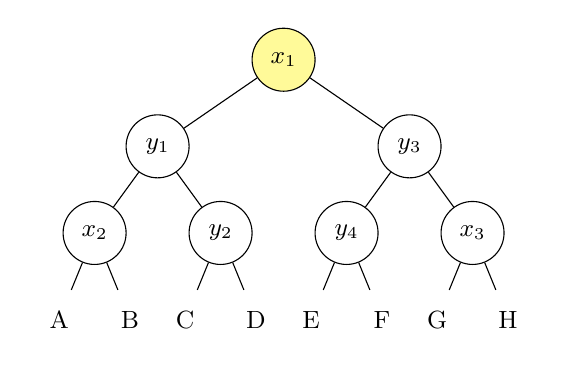
\begin{tikzpicture}[
  level distance=1.1cm,
  level 1/.style={sibling distance=3.2cm},
  level 2/.style={sibling distance=1.6cm},
  level 3/.style={sibling distance=0.9cm},
  every node/.style={circle, draw, minimum size=8mm, inner sep=1pt, font=\small},
  edge from parent/.style={draw,-}
]
\node[fill=yellow!40] {$x_1$}
  child { node {$y_1$}
    child { node {$x_2$}
      child { node[draw=none] {A} }
      child { node[draw=none] {B} }
    }
    child { node {$y_2$}
      child { node[draw=none] {C} }
      child { node[draw=none] {D} }
    }
  }
  child { node {$y_3$}
    child { node {$y_4$}
      child { node[draw=none] {E} }
      child { node[draw=none] {F} }
    }
    child { node {$x_3$}
      child { node[draw=none] {G} }
      child { node[draw=none] {H} }
    }
  };
\end{tikzpicture}
\end{minipage}%
\begin{minipage}{0.4\textwidth}
\centering
\includegraphics[width=\textwidth]{images/kdtreerange.png}
\end{minipage}
\end{center}

\textbf{Step 2: Search left child ($y_1$)}

This node splits on y. We check:
\begin{itemize}
    \item Is $y_s \leq y_1$? \textbf{No} $\rightarrow$ don't search left child
    \item Is $y_e \geq y_1$? \textbf{Yes} $\rightarrow$ search right child
\end{itemize}

The range is entirely above $y_1$, so we only search the right child. This prunes the entire lower-left region (points A and B).

\begin{center}
\begin{minipage}{0.55\textwidth}
\centering
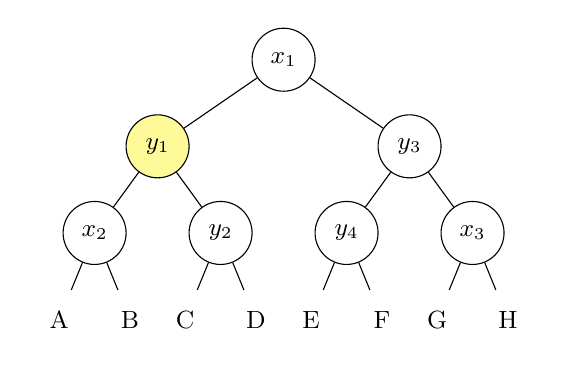
\begin{tikzpicture}[
  level distance=1.1cm,
  level 1/.style={sibling distance=3.2cm},
  level 2/.style={sibling distance=1.6cm},
  level 3/.style={sibling distance=0.9cm},
  every node/.style={circle, draw, minimum size=8mm, inner sep=1pt, font=\small},
  edge from parent/.style={draw,-}
]
\node {$x_1$}
  child { node[fill=yellow!40] {$y_1$}
    child { node {$x_2$}
      child { node[draw=none] {A} }
      child { node[draw=none] {B} }
    }
    child { node {$y_2$}
      child { node[draw=none] {C} }
      child { node[draw=none] {D} }
    }
  }
  child { node {$y_3$}
    child { node {$y_4$}
      child { node[draw=none] {E} }
      child { node[draw=none] {F} }
    }
    child { node {$x_3$}
      child { node[draw=none] {G} }
      child { node[draw=none] {H} }
    }
  };
\end{tikzpicture}
\end{minipage}%
\begin{minipage}{0.4\textwidth}
\centering
\includegraphics[width=\textwidth]{images/kdtreerange.png}
\end{minipage}
\end{center}

\textbf{Step 3: Search $y_1$'s right child ($y_2$)}

This node splits on y. We check:
\begin{itemize}
    \item Is $y_s \leq y_2$? \textbf{Yes} $\rightarrow$ search left child (point C)
    \item Is $y_e \geq y_2$? \textbf{Yes} $\rightarrow$ search right child (point D)
\end{itemize}

At leaf C, check if C is in range: \textbf{Yes!} C is \textbf{in range}.

At leaf D, check if D is in range: \textbf{Yes!} D is \textbf{in range}.

\begin{center}
\begin{minipage}{0.55\textwidth}
\centering
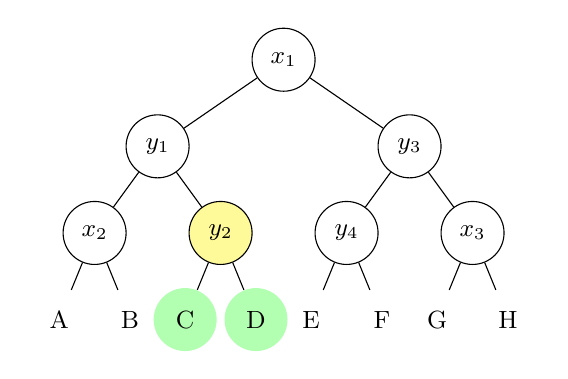
\begin{tikzpicture}[
  level distance=1.1cm,
  level 1/.style={sibling distance=3.2cm},
  level 2/.style={sibling distance=1.6cm},
  level 3/.style={sibling distance=0.9cm},
  every node/.style={circle, draw, minimum size=8mm, inner sep=1pt, font=\small},
  edge from parent/.style={draw,-}
]
\node {$x_1$}
  child { node {$y_1$}
    child { node {$x_2$}
      child { node[draw=none] {A} }
      child { node[draw=none] {B} }
    }
    child { node[fill=yellow!40] {$y_2$}
      child { node[draw=none,fill=green!30] {C} }
      child { node[draw=none,fill=green!30] {D} }
    }
  }
  child { node {$y_3$}
    child { node {$y_4$}
      child { node[draw=none] {E} }
      child { node[draw=none] {F} }
    }
    child { node {$x_3$}
      child { node[draw=none] {G} }
      child { node[draw=none] {H} }
    }
  };
\end{tikzpicture}
\end{minipage}%
\begin{minipage}{0.4\textwidth}
\centering
\includegraphics[width=\textwidth]{images/kdtreerange.png}
\end{minipage}
\end{center}

\textbf{Step 4: Back to root, search right child ($y_3$)}

Now we explore the right subtree of the root. This node splits on y. We check:
\begin{itemize}
    \item Is $y_s \leq y_3$? \textbf{No} $\rightarrow$ don't search left child
    \item Is $y_e \geq y_3$? \textbf{Yes} $\rightarrow$ search right child
\end{itemize}

The range is entirely above $y_3$, so we only search the right child. This prunes the lower-right region (points E and F).

\begin{center}
\begin{minipage}{0.55\textwidth}
\centering
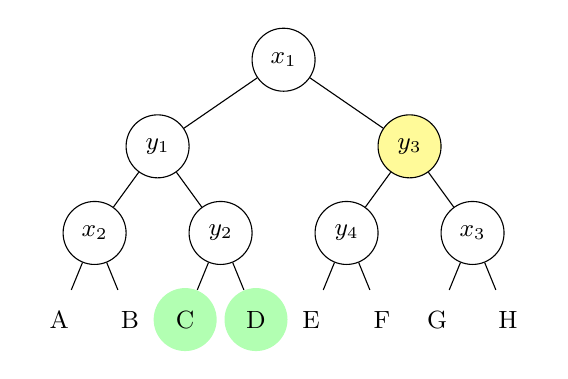
\begin{tikzpicture}[
  level distance=1.1cm,
  level 1/.style={sibling distance=3.2cm},
  level 2/.style={sibling distance=1.6cm},
  level 3/.style={sibling distance=0.9cm},
  every node/.style={circle, draw, minimum size=8mm, inner sep=1pt, font=\small},
  edge from parent/.style={draw,-}
]
\node {$x_1$}
  child { node {$y_1$}
    child { node {$x_2$}
      child { node[draw=none] {A} }
      child { node[draw=none] {B} }
    }
    child { node {$y_2$}
      child { node[draw=none,fill=green!30] {C} }
      child { node[draw=none,fill=green!30] {D} }
    }
  }
  child { node[fill=yellow!40] {$y_3$}
    child { node {$y_4$}
      child { node[draw=none] {E} }
      child { node[draw=none] {F} }
    }
    child { node {$x_3$}
      child { node[draw=none] {G} }
      child { node[draw=none] {H} }
    }
  };
\end{tikzpicture}
\end{minipage}%
\begin{minipage}{0.4\textwidth}
\centering
\includegraphics[width=\textwidth]{images/kdtreerange.png}
\end{minipage}
\end{center}

\textbf{Step 5: Search $y_3$'s right child ($x_3$)}

This node splits on x. We check:
\begin{itemize}
    \item Is $x_s \leq x_3$? \textbf{Yes} $\rightarrow$ search left child (point G)
    \item Is $x_e \geq x_3$? \textbf{No} $\rightarrow$ don't search right child
\end{itemize}

At leaf G, check if G is in range: \textbf{Yes!} G is \textbf{in range}.

We don't need to check H because the range doesn't extend past $x_3$.

\begin{center}
\begin{minipage}{0.55\textwidth}
\centering
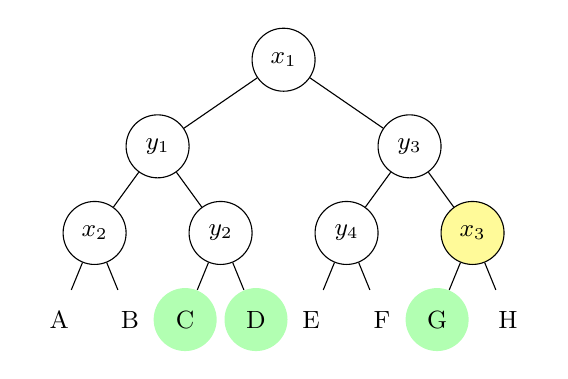
\begin{tikzpicture}[
  level distance=1.1cm,
  level 1/.style={sibling distance=3.2cm},
  level 2/.style={sibling distance=1.6cm},
  level 3/.style={sibling distance=0.9cm},
  every node/.style={circle, draw, minimum size=8mm, inner sep=1pt, font=\small},
  edge from parent/.style={draw,-}
]
\node {$x_1$}
  child { node {$y_1$}
    child { node {$x_2$}
      child { node[draw=none] {A} }
      child { node[draw=none] {B} }
    }
    child { node {$y_2$}
      child { node[draw=none,fill=green!30] {C} }
      child { node[draw=none,fill=green!30] {D} }
    }
  }
  child { node {$y_3$}
    child { node {$y_4$}
      child { node[draw=none] {E} }
      child { node[draw=none] {F} }
    }
    child { node[fill=yellow!40] {$x_3$}
      child { node[draw=none,fill=green!30] {G} }
      child { node[draw=none] {H} }
    }
  };
\end{tikzpicture}
\end{minipage}%
\begin{minipage}{0.4\textwidth}
\centering
\includegraphics[width=\textwidth]{images/kdtreerange.png}
\end{minipage}
\end{center}

\textbf{Final Result:} Points in range: \textbf{C, D, G}

\subsubsection*{Why Must We Check at the Leaf?}

Reaching a leaf does \textbf{not} guarantee the point is in range. Each split only checks \textbf{one dimension} at a time:
\begin{itemize}
    \item An x-split filters based on x only
    \item A y-split filters based on y only
\end{itemize}

We don't verify both dimensions together until we reach the leaf. For example, point B was reached because the range overlapped its region, but B's actual y-coordinate was outside $[y_s, y_e]$.

The cost of range search depends on how many branches we must explore:

\[
\text{Cost} = (\log_2(B \cdot R) + 1) \cdot (\text{number of matching pages}) \cdot D
\]

\begin{itemize}
    \item \textbf{Best case:} The range is small and falls entirely within one region at each level. We follow a single path down, similar to point lookup.
    \item \textbf{Worst case:} The range covers most of the space, and we must visit nearly all nodes (degrades to a full scan).
    \item \textbf{Typical case:} Pruning eliminates large portions of the tree. In our example, we skipped A, B, E, F, and H entirely.
\end{itemize}

The actual cost depends on how large the range is relative to the data distribution.

\subsection{Nearest Neighbor Search}

Nearest neighbor search finds the closest point to a given query point $P$. This is useful for applications like finding the nearest star to a location, or the closest monster to a game character.

\textbf{Naive approach:} Scan all points and compute the distance to each one. Cost: $B \cdot D$ (full table scan).

\textbf{Better approach:} Use the KD tree to prune regions that cannot contain a closer point.

\textbf{Algorithm:}
\begin{enumerate}
    \item Traverse down the tree as if inserting $P$, keeping track of the closest point found so far.
    \item At each leaf, check if the point is closer than the current best.
    \item \textbf{Backtrack} up the tree, checking if other branches could contain a closer point.
    \item Use geometry to prune: if the closest possible point in a region is farther than the current best, skip that entire branch.
\end{enumerate}

\textbf{Key insight:} We can avoid searching entire subtrees by computing the minimum possible distance from $P$ to any point in that region. If this minimum distance exceeds our current best, there's no point searching there.

\subsubsection*{Step-by-Step Example}

Using the KD tree from construction, suppose we want to find the nearest neighbor to point $P$ (the red square in the figure).

\textbf{Step 1: Traverse down as if inserting $P$}

Starting at the root ($x_1$), we compare $P.x$ with $x_1$. Since $P.x > x_1$, we go right to $y_3$.

At $y_3$, we compare $P.y$ with $y_3$. Since $P.y < y_3$, we go left to $y_4$.

At $y_4$, we compare $P.y$ with $y_4$. Since $P.y < y_4$, we go left to $E$.

We've reached leaf $E$. Set $E$ as our current best.

\begin{center}
\begin{minipage}{0.55\textwidth}
\centering
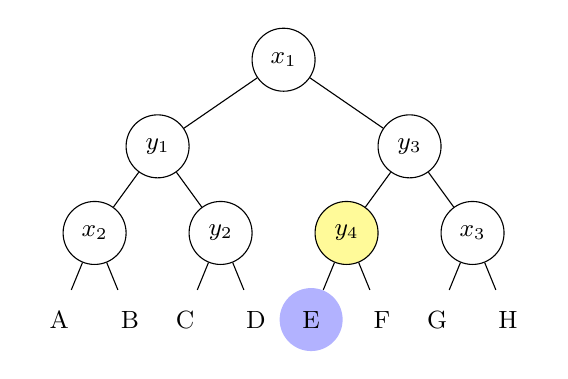
\begin{tikzpicture}[
  level distance=1.1cm,
  level 1/.style={sibling distance=3.2cm},
  level 2/.style={sibling distance=1.6cm},
  level 3/.style={sibling distance=0.9cm},
  every node/.style={circle, draw, minimum size=8mm, inner sep=1pt, font=\small},
  edge from parent/.style={draw,-}
]
\node {$x_1$}
  child { node {$y_1$}
    child { node {$x_2$}
      child { node[draw=none] {A} }
      child { node[draw=none] {B} }
    }
    child { node {$y_2$}
      child { node[draw=none] {C} }
      child { node[draw=none] {D} }
    }
  }
  child { node {$y_3$}
    child { node[fill=yellow!40] {$y_4$}
      child { node[draw=none,fill=blue!30] {E} }
      child { node[draw=none] {F} }
    }
    child { node {$x_3$}
      child { node[draw=none] {G} }
      child { node[draw=none] {H} }
    }
  };
\end{tikzpicture}
\end{minipage}%
\begin{minipage}{0.4\textwidth}
\centering
\includegraphics[width=\textwidth]{images/nearestNeighbour.png}
\end{minipage}
\end{center}

\textbf{Step 2: Backtrack to $y_4$, check sibling $F$}

We backtrack to $y_4$ and check if the other child ($F$) could contain a closer point.

The region containing $F$ is above $y_4$. We compute the minimum distance from $P$ to this region. Since $F$ is closer to $P$ than $E$, we update our best to $F$.

\begin{center}
\begin{minipage}{0.55\textwidth}
\centering
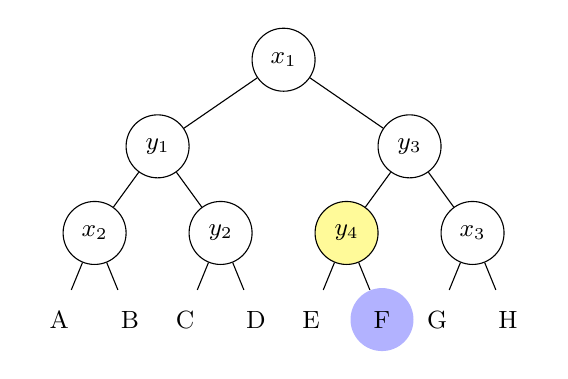
\begin{tikzpicture}[
  level distance=1.1cm,
  level 1/.style={sibling distance=3.2cm},
  level 2/.style={sibling distance=1.6cm},
  level 3/.style={sibling distance=0.9cm},
  every node/.style={circle, draw, minimum size=8mm, inner sep=1pt, font=\small},
  edge from parent/.style={draw,-}
]
\node {$x_1$}
  child { node {$y_1$}
    child { node {$x_2$}
      child { node[draw=none] {A} }
      child { node[draw=none] {B} }
    }
    child { node {$y_2$}
      child { node[draw=none] {C} }
      child { node[draw=none] {D} }
    }
  }
  child { node {$y_3$}
    child { node[fill=yellow!40] {$y_4$}
      child { node[draw=none] {E} }
      child { node[draw=none,fill=blue!30] {F} }
    }
    child { node {$x_3$}
      child { node[draw=none] {G} }
      child { node[draw=none] {H} }
    }
  };
\end{tikzpicture}
\end{minipage}%
\begin{minipage}{0.4\textwidth}
\centering
\includegraphics[width=\textwidth]{images/nearestNeighbour.png}
\end{minipage}
\end{center}

\textbf{Step 3: Backtrack to $y_3$, check sibling subtree ($x_3$)}

We backtrack to $y_3$ and check if the region above $y_3$ (containing $G$ and $H$) could have a closer point.

The minimum distance from $P$ to this upper-right region is greater than the distance from $P$ to $F$. Therefore, we \textbf{prune} this entire subtree—no need to check $G$ or $H$.

\begin{center}
\begin{minipage}{0.55\textwidth}
\centering
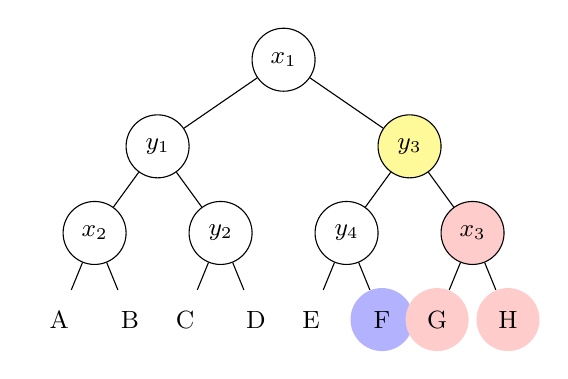
\begin{tikzpicture}[
  level distance=1.1cm,
  level 1/.style={sibling distance=3.2cm},
  level 2/.style={sibling distance=1.6cm},
  level 3/.style={sibling distance=0.9cm},
  every node/.style={circle, draw, minimum size=8mm, inner sep=1pt, font=\small},
  edge from parent/.style={draw,-}
]
\node {$x_1$}
  child { node {$y_1$}
    child { node {$x_2$}
      child { node[draw=none] {A} }
      child { node[draw=none] {B} }
    }
    child { node {$y_2$}
      child { node[draw=none] {C} }
      child { node[draw=none] {D} }
    }
  }
  child { node[fill=yellow!40] {$y_3$}
    child { node {$y_4$}
      child { node[draw=none] {E} }
      child { node[draw=none,fill=blue!30] {F} }
    }
    child { node[fill=red!20] {$x_3$}
      child { node[draw=none,fill=red!20] {G} }
      child { node[draw=none,fill=red!20] {H} }
    }
  };
\end{tikzpicture}
\end{minipage}%
\begin{minipage}{0.4\textwidth}
\centering
\includegraphics[width=\textwidth]{images/nearestNeighbour.png}
\end{minipage}
\end{center}

\textbf{Step 4: Backtrack to root, check left subtree ($y_1$)}

We backtrack to the root ($x_1$) and check if the left half of the space could contain a closer point.

We traverse down to $y_1$. The region below $y_1$ (containing $A$ and $B$) could potentially have a closer point, so we check it.

At $x_2$, we find that $B$ is closer to $P$ than $F$! Update our best to $B$.

\begin{center}
\begin{minipage}{0.55\textwidth}
\centering
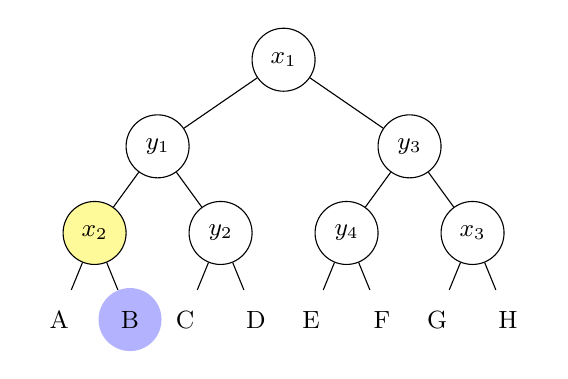
\begin{tikzpicture}[
  level distance=1.1cm,
  level 1/.style={sibling distance=3.2cm},
  level 2/.style={sibling distance=1.6cm},
  level 3/.style={sibling distance=0.9cm},
  every node/.style={circle, draw, minimum size=8mm, inner sep=1pt, font=\small},
  edge from parent/.style={draw,-}
]
\node {$x_1$}
  child { node {$y_1$}
    child { node[fill=yellow!40] {$x_2$}
      child { node[draw=none] {A} }
      child { node[draw=none,fill=blue!30] {B} }
    }
    child { node {$y_2$}
      child { node[draw=none] {C} }
      child { node[draw=none] {D} }
    }
  }
  child { node {$y_3$}
    child { node {$y_4$}
      child { node[draw=none] {E} }
      child { node[draw=none] {F} }
    }
    child { node {$x_3$}
      child { node[draw=none] {G} }
      child { node[draw=none] {H} }
    }
  };
\end{tikzpicture}
\end{minipage}%
\begin{minipage}{0.4\textwidth}
\centering
\includegraphics[width=\textwidth]{images/nearestNeighbour.png}
\end{minipage}
\end{center}

\textbf{Step 5: Check if upper-left region could have closer point}

We check if the region above $y_1$ (containing $C$ and $D$) could have a closer point than $B$.

The minimum distance from $P$ to this region is greater than the distance from $P$ to $B$. Therefore, we \textbf{prune} this subtree—no need to check $C$ or $D$.

\begin{center}
\begin{minipage}{0.55\textwidth}
\centering
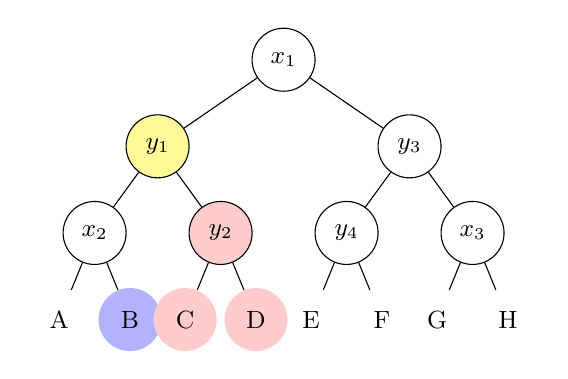
\begin{tikzpicture}[
  level distance=1.1cm,
  level 1/.style={sibling distance=3.2cm},
  level 2/.style={sibling distance=1.6cm},
  level 3/.style={sibling distance=0.9cm},
  every node/.style={circle, draw, minimum size=8mm, inner sep=1pt, font=\small},
  edge from parent/.style={draw,-}
]
\node {$x_1$}
  child { node[fill=yellow!40] {$y_1$}
    child { node {$x_2$}
      child { node[draw=none] {A} }
      child { node[draw=none,fill=blue!30] {B} }
    }
    child { node[fill=red!20] {$y_2$}
      child { node[draw=none,fill=red!20] {C} }
      child { node[draw=none,fill=red!20] {D} }
    }
  }
  child { node {$y_3$}
    child { node {$y_4$}
      child { node[draw=none] {E} }
      child { node[draw=none] {F} }
    }
    child { node {$x_3$}
      child { node[draw=none] {G} }
      child { node[draw=none] {H} }
    }
  };
\end{tikzpicture}
\end{minipage}%
\begin{minipage}{0.4\textwidth}
\centering
\includegraphics[width=\textwidth]{images/nearestNeighbour.png}
\end{minipage}
\end{center}

\textbf{Final Result:} Nearest neighbor to $P$ is \textbf{B}.

\subsubsection*{How Pruning Works}

To decide whether to search a region, we compute the \textbf{minimum possible distance} from $P$ to any point in that region:

\begin{itemize}
    \item For a region defined by split lines, find the closest point on the region's boundary to $P$.
    \item If this minimum distance is greater than the distance to our current best, skip the entire region.
\end{itemize}

In geometric terms, imagine drawing a circle around $P$ with radius equal to the distance to the current best. If a region doesn't intersect this circle, it cannot contain a closer point.

\subsubsection*{Key Observations}

\begin{itemize}
    \item \textbf{Pruning saves work:} We skipped $G$, $H$, $C$, and $D$ entirely because their regions couldn't contain a closer point.
    \item \textbf{Order matters:} The initial traversal path affects how quickly we find a good candidate. A closer initial guess leads to more pruning.
    \item \textbf{Must backtrack:} Unlike range search, we can't just follow one path. The nearest neighbor might be in a different branch than where $P$ would be inserted.
    \item \textbf{Worst case:} If points are distributed poorly, we may need to visit many nodes. But typically, pruning eliminates large portions of the tree.
\end{itemize}

\subsubsection*{I/O Cost}

The cost depends on how much pruning occurs:

\begin{itemize}
    \item \textbf{Best case:} The nearest neighbor is found on the initial traversal, and all other branches are pruned. Cost: $(\log_2(B \cdot R) + 2) \cdot D$ (same as point lookup).
    \item \textbf{Worst case:} Little pruning occurs, and we visit most nodes. Cost approaches $B \cdot D$ (full scan).
    \item \textbf{Typical case:} Pruning eliminates most branches. Cost is a small multiple of $\log_2(B \cdot R)$.
\end{itemize}

\subsection{Insertion and Deletion}

To insert a new point, traverse to find where it belongs, then add it.

\[
\text{Cost} = (\log_2(B \cdot R) + 4) \cdot D
\]

\begin{itemize}
    \item $\log_2(B \cdot R) + 1$: traverse down the tree (the $+1$ adjusts for the fact that $\log_2(n)$ gives levels minus one)
    \item $+3$: read the data page, write the data page, and write a new index node
\end{itemize}

To delete a point, find it first, then remove it.

\[
\text{Cost} = (\log_2(B \cdot R) + 4) \cdot D
\]

\begin{itemize}
    \item $\log_2(B \cdot R) + 1$: traverse down the tree
    \item $+3$: read the data page, write the modified data page, and potentially update an index node
\end{itemize}

Unlike B+ trees, KD trees do not have splitting or merging operations to maintain balance. Repeated insertions and deletions can cause the tree to become unbalanced, leading to deeper traversals and worse query performance. This is why databases typically \textbf{bulk load} KD trees.

\subsection{I/O Cost Summary}

\begin{table}[H]
    \centering
    \begin{tabular}{lc}
        \toprule
        \textbf{Operation} & \textbf{KD Tree} \\
        \midrule
        Scan all records & $B \cdot D$ \\
        Point Lookup & $(\log_2(B \cdot R) + 2) \cdot D$ \\
        Range Search & $(\log_2(B \cdot R) + 1) \cdot \text{pages} \cdot D$ \\
        Insert & $(\log_2(B \cdot R) + 4) \cdot D$ \\
        Delete & $(\log_2(B \cdot R) + 4) \cdot D$ \\
        \bottomrule
    \end{tabular}
    \caption{KD Tree I/O cost (in page reads)}
\end{table}